% If I add all results to the Evaluation chapter, there's no need for a Results chapter.

% This will depend on how I structure the document once I start writing the experiments and results sections. For now, this stays empty.

\chapter{Results and Discussion}
In this chapter, the results from the experiment will be discussed.

\section{Results}
This section will introduce the results from the experiments.

\subsection{Masking Ratio for Masked Language Modeling}
The results from masking ratio for \acrshort{mlm} is shown on table \ref{tb:fixed_mlm}. From table \ref{tb:fixed_mlm} the metric measures the percentage of times the correct image is among the top K retrieved images for a given text query. Common values for K include 1, 5, and 10, represented as R@1, R@5, and R@10 respectively. The highest results for each metrics are shown bold.

\subsubsection{Fixed Masking Ratio}
The results from table \ref{tb:fixed_mlm} shows that prediction accuracy differs below 2\%. For R@1 masking ratio of 30\% had the highest accuracy, but 15\% marked the highest for r@5 and r@10. 0.3~0.55\% difference was observed from the results in table \ref{tb:fixed_mlm}, and no change in performance was observed by changing the mask rate.

\begin{table}[htbp]
    \centering
    \caption{Result for masking fixed masking ratio}
    \label{tb:fixed_mlm}
    
    \begin{tabular}{rcccc}
      masking ratio & r@1 & r@5 & r@10 & mAP\\ \hline
      15\% & 76.51 & \textbf{90.20} & \textbf{94.25} & 69.38 \\
      20\% & 76.64 & 89.90 & 93.70 & 70.27 \\
      25\% & 76.23 & 89.86 & 93.79 & 70.22 \\
      30\% & \textbf{76.72} & 89.77 & 93.60 & \textbf{70.30} \\
      35\% & 76.61 & 89.77 & 93.47 & 70.26 \\
      40\% & 76.56 & 89.88 & 93.47 & 70.26
    \end{tabular}
\end{table}

\subsubsection{Timevariant Masking Ratio}
\begin{table}[htbp]
  \centering
  \caption{Result for time variant masking ratio}
  \label{tb:time_variant_mlm}
  \begin{tabular}{rcccc}
    \centering
    masking ratio & r@1 & r@5 & r@10 & mAP\\ \hline
    linear increase & 76.62 & 89.88 & 93.62 & \textbf{70.36} \\
    linear decrease & \textbf{76.70} & 89.85 & 93.58 & 70.21 \\
    cosine increase & 76.54 & 90.04 & \textbf{94.02} & 70.15 \\
    cosine decrease & 76.21 & \textbf{90.09} & 93.65 & 70.21 \\
  \end{tabular}
\end{table}


\subsection{Masking Ratio for Momentum-based Replaced Token Detection}

\subsubsection{Fixed Masking Ratio}
\begin{figure}
    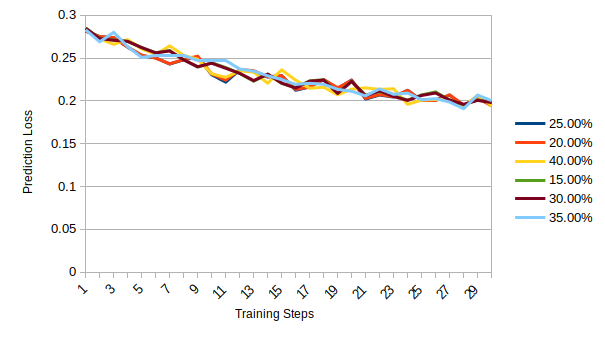
\includegraphics[width=\linewidth]{img/mrtd_prd_loss.png}
    \caption{Prediction loss in training steps}
    \label{img:mrtd_prd_loss}
\end{figure}

\begin{figure}
    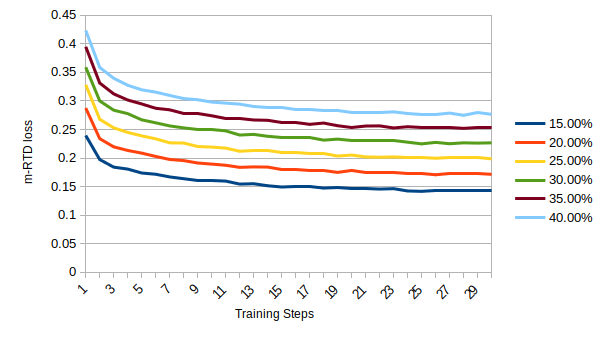
\includegraphics[width=\linewidth]{img/mrtd_loss.png}
    \caption{MRTD Loss in training steps}
    \label{img:mrtd_loss}
\end{figure}

\begin{table}[htbp]
  \centering
  \caption{Result for fixed masking ratio on m-RTD}
  \begin{tabular}{rcccc}
    masking ratio & r@1 & r@5 & r@10 & mAP \\ \hline
    15\% & 75.42 & 90.20 & 93.83 & 68.56 \\
    20\% & 75.58 & 90.35 & 93.91 & 68.73 \\
    25\% & 75.63 & 90.09 & 93.83 & 68.76 \\
    30\% & 75.57 & \textbf{93.92} & 93.92 & \textbf{68.81} \\
    35\% & 75.03 & 90.14 & 93.89 & 68.57 \\
    40\% & \textbf{75.80} & 90.27 & \textbf{93.97} & 68.73
  \end{tabular}
\end{table}

\subsubsection{Time Variant Masking Ratio}
\begin{table}[htbp]
  \centering
  \caption{Result for time variant masking ratio}
  \begin{tabular}{rcccc}
    \centering
    masking ratio & r@1 & r@5 & r@10 & mAP\\ \hline
    linear increase & 76.20 & 90.11 & 93.94 & 70.22 \\
    linear decrease & \textbf{76.70} & 89.85 & 93.58 & 70.21 \\
    cosine increase & 75.91 & 89.85 & 93.89 & 68.40 \\
    cosine decrease & 75.99 & 90.25 & 94.01 & 68.73 \\
  \end{tabular}
\end{table}


\section{Discussion}
\subsection{Impact of Masking Ratio}

The experiments demonstrate that the effect of changing the masking ratio trivial towards the performance of \acrshort{rasa}. 
The effect of prediction for different masking ratio has been researched by \cite{yang2023learningbettermaskingbetter} in pre-training steps, which they used for \acrshort{nlp} tasks. However, there are no papers which evaluates in the fine-tuning step so far.


The experiments demonstrate that the effect of changing the masking ratio trivial towards the performance of \acrshort{rasa}. From Table\ref{tb:fixed_mlm} shows that the prediction does not change at all. \cite{yang2023learningbettermaskingbetter} did a work of changing the masking ratio at pre-training task, but no other papers worked on changing the masking ratio on fine-tuning phase. 
Although \cite{yang2023learningbettermaskingbetter} pointed out that their work gave significant improvements in pre-training phase, but the results from our experiment tells that changing the masking ratio on fine-tuning part does not make an improvements with different masking ratio.
From Table\ref{tb:fixed_mlm}, the 

The experiments demonstrate that the masking ratio plays a significant role in the performance of VLMs. A fixed masking ratio, while effective, may not provide the optimal balance needed for different stages of training. The introduction of a time-variant masking ratio allows the model to adaptively focus on different aspects of the data, potentially enhancing its ability to learn robust representations. This adaptive approach appears to improve the model's capacity to handle the complexities inherent in text-based person retrieval tasks.
The results are not the way we expected to have. \acrshort{mlm} is the important loss function towards \acrshort{vlm} and NLP models. 


\section{Training Metrics}

The analysis of training dynamics reveals that varying the masking ratio affects the learning process in nuanced ways. With a higher masking ratio, the model is forced to infer more missing information, which can lead to better generalization but at the cost of increased computational complexity. Conversely, lower masking ratios may result in faster convergence but could limit the model's ability to learn comprehensive representations. The trade-off between inference accuracy and computational efficiency is a critical consideration in the design of effective VLMs.

\section{Fine Tuning and Pre Training}

The results underscore the importance of the fine-tuning phase in aligning the pre-trained VLMs to specific tasks. While the pre-training phase establishes a robust foundational knowledge base, fine-tuning optimizes the model for task-specific performance. The experiments indicate that fine-tuning with a well-designed masking strategy can significantly enhance the accuracy of text-based person retrieval models.


% -- results line 
% talk about my work
%   check the numbers, use the visual grounding 
%   - training loss Graph
%   the results shows the loss prd, masking ratio, and loss mlm.
%   loss mlm correlates to the masking ratio, but prd decrease the same way for all 
%   - evaluation 
%   the r1~r10 does not change at all 

% -- discussion line
% discuss about the prediction 
% - my work didn't change at all 
% - for mlm, this method is major task for NLP and VLM models
% - previous method did an analysis in pre-training steps, which made significant difference because it's the part where the model actually learns how to achieve information from the modality
% - in fine-tuning, they're trained to generate the answers which corresponds to specific tasks
% - it's just fitting the model to specific method which does not effect that much to the actual model knowledge, that's why the fine-tuning part is more important to have better training task that really fits to the task you want the model to solve <- this requires good reference to explain. use the rasa results and the results i have
%   also use the visual grounding as well 


%   Training Loss Analysis: The study examines the correlation between the masking ratio and the training loss for masked language modeling. It is observed that while the prediction loss (prd) decreases consistently, the loss associated with MLM varies according to the masking ratio.
% Evaluation Metrics: Metrics such as R1 (Recall at 1) and R10 (Recall at 10) are utilized to measure the effectiveness of different masking ratios. The results indicate that these evaluation metrics do not exhibit significant changes despite varying masking ratios.
% Importance of Fine-Tuning: The discussion emphasizes that the primary learning phase for VLMs is during pre-training, where the model learns to extract information from different modalities. Fine-tuning, on the other hand, aligns the model to specific tasks and does not significantly alter the foundational knowledge acquired during pre-training.
% Comparison with Previous Methods: The paper contrasts the current approach with previous methods that analyzed masking ratios in pre-training steps. It suggests that fine-tuning plays a critical role in achieving task-specific accuracy, and thus, having a well-designed fine-tuning task is crucial for the model's performance.

